\documentclass[12pt, a4paper]{article}

\usepackage{graphicx}
\usepackage{float}
\usepackage{subfig}
\usepackage[left=.75in,top=.75in,right=.75in,bottom=.75in]{geometry}

\begin{document} 

\section{rat}
\begin{figure}[H]
\centerline{
\subfloat[DSD vs Density]{
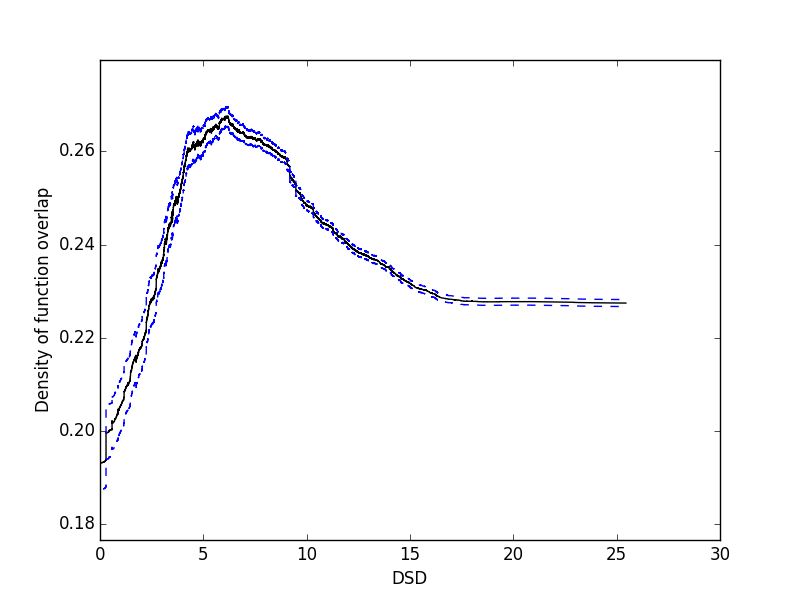
\includegraphics[width=0.333333333333\textwidth]{plots/rat_dsd_density.png}
}
\subfloat[DSD vs Overlap, Pairs]{
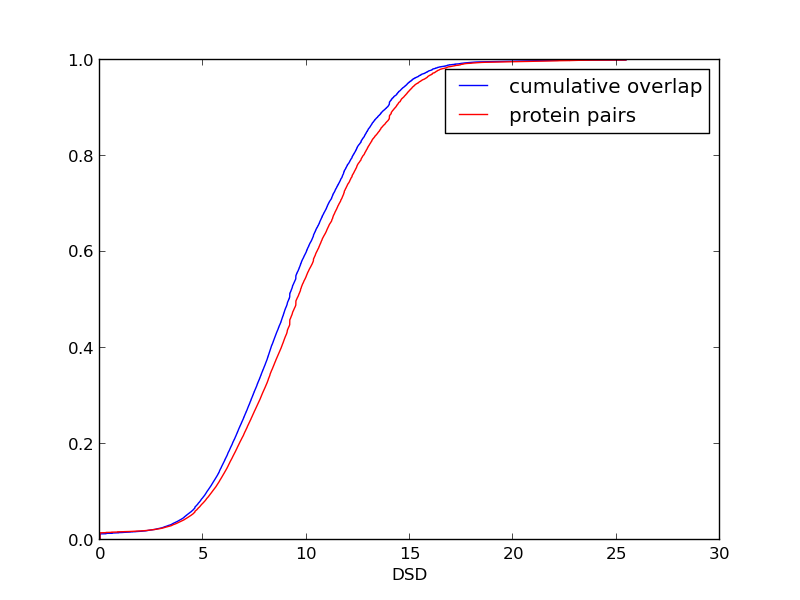
\includegraphics[width=0.333333333333\textwidth]{plots/rat_dsd_overlap_pairs.png}
}
\subfloat[Pairs vs Cumulative Overlap]{
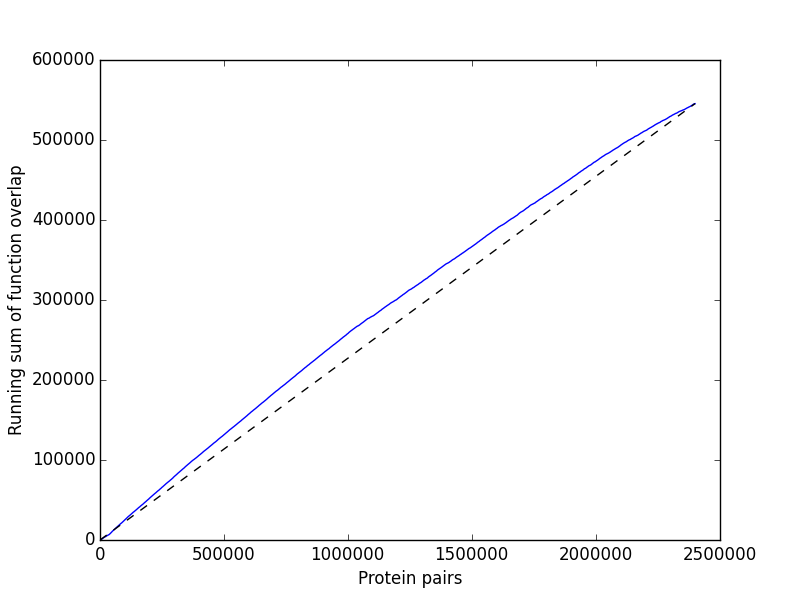
\includegraphics[width=0.333333333333\textwidth]{plots/rat_pairs_overlap.png}
}
}
\end{figure}

\subsection{Plots based on random permutation of label sets}
\begin{figure}[H]
\centerline{
\subfloat[DSD vs Density]{
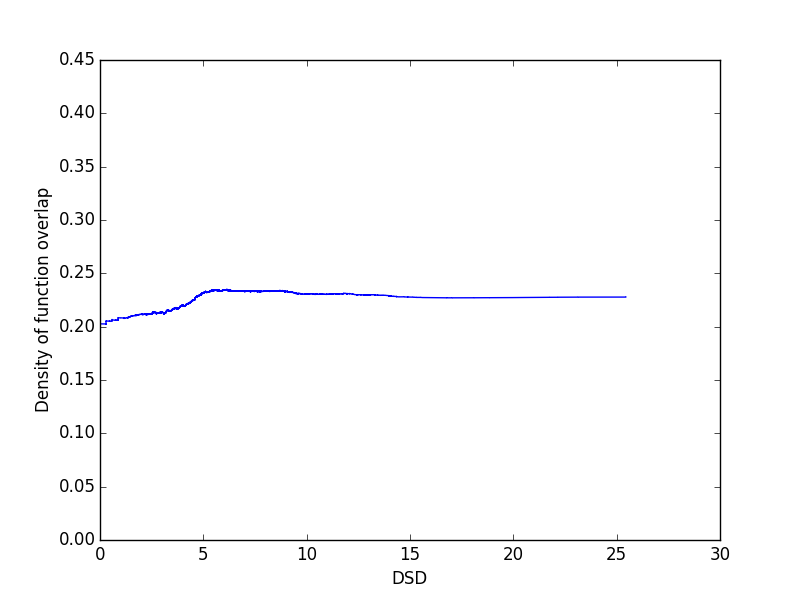
\includegraphics[width=0.333333333333\textwidth]{plots/rat_dsd_density_randomized.png}
}
\subfloat[DSD vs Overlap, Pairs]{
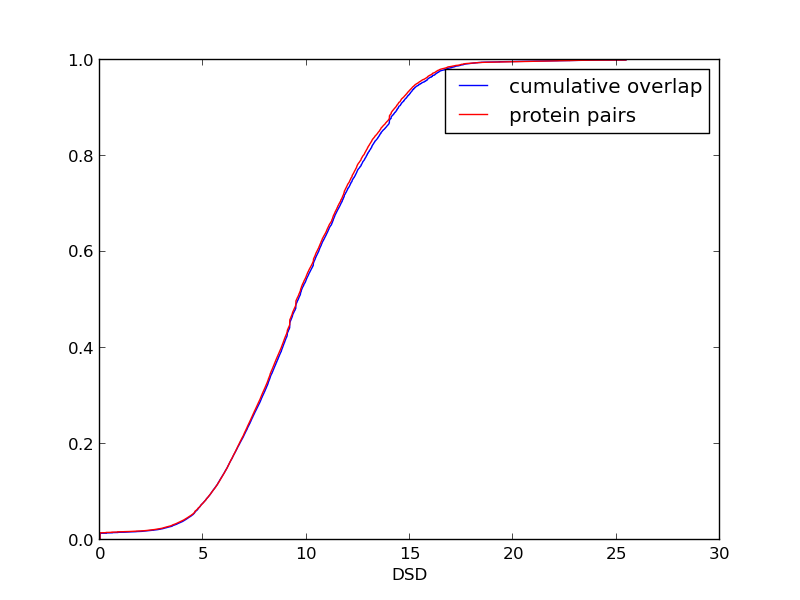
\includegraphics[width=0.333333333333\textwidth]{plots/rat_dsd_overlap_pairs_randomized.png}
}
\subfloat[Pairs vs Cumulative Overlap]{
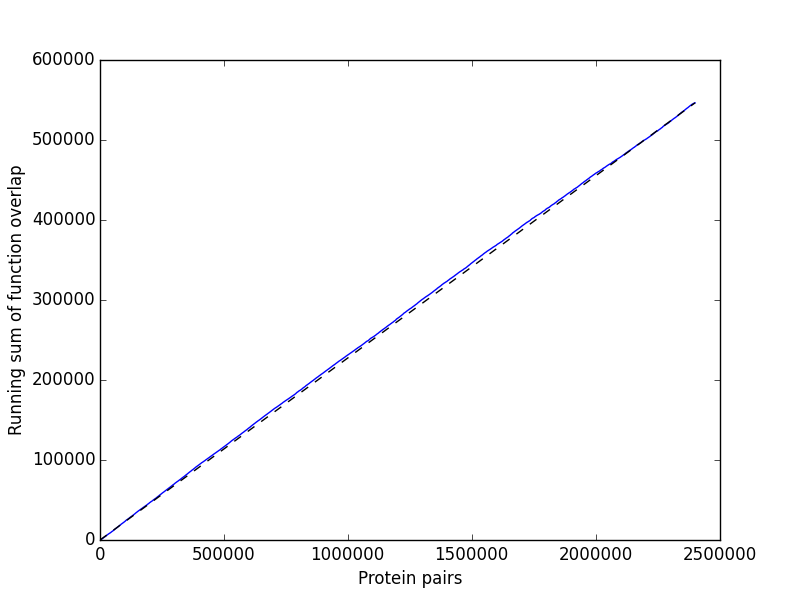
\includegraphics[width=0.333333333333\textwidth]{plots/rat_pairs_overlap_randomized.png}
}
}
\end{figure}

\section{mouse}
\begin{figure}[H]
\centerline{
\subfloat[DSD vs Density]{
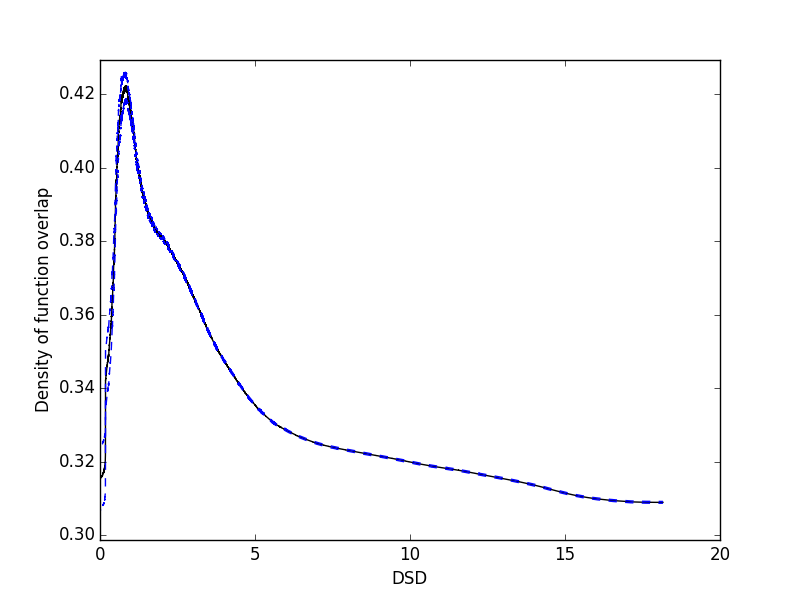
\includegraphics[width=0.333333333333\textwidth]{plots/mouse_dsd_density.png}
}
\subfloat[DSD vs Overlap, Pairs]{
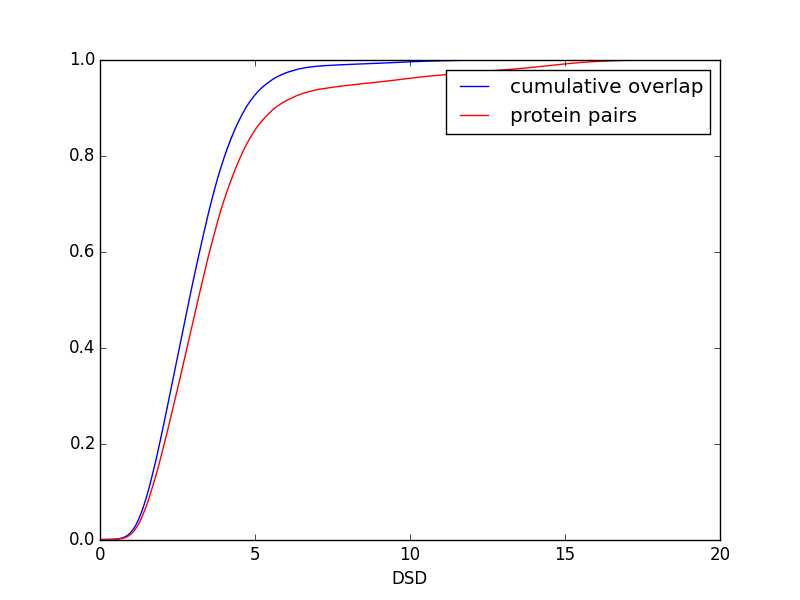
\includegraphics[width=0.333333333333\textwidth]{plots/mouse_dsd_overlap_pairs.png}
}
\subfloat[Pairs vs Cumulative Overlap]{
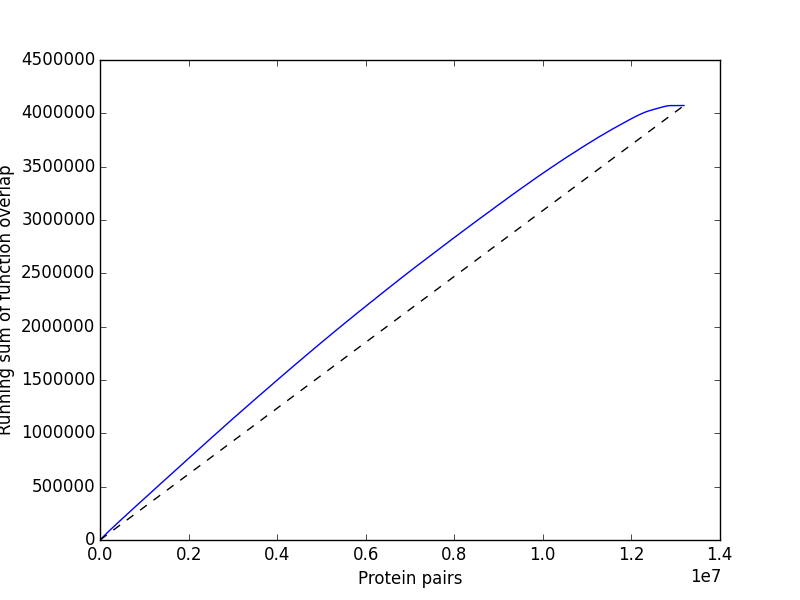
\includegraphics[width=0.333333333333\textwidth]{plots/mouse_pairs_overlap.png}
}
}
\end{figure}

\subsection{Plots based on random permutation of label sets}
\begin{figure}[H]
\centerline{
\subfloat[DSD vs Density]{
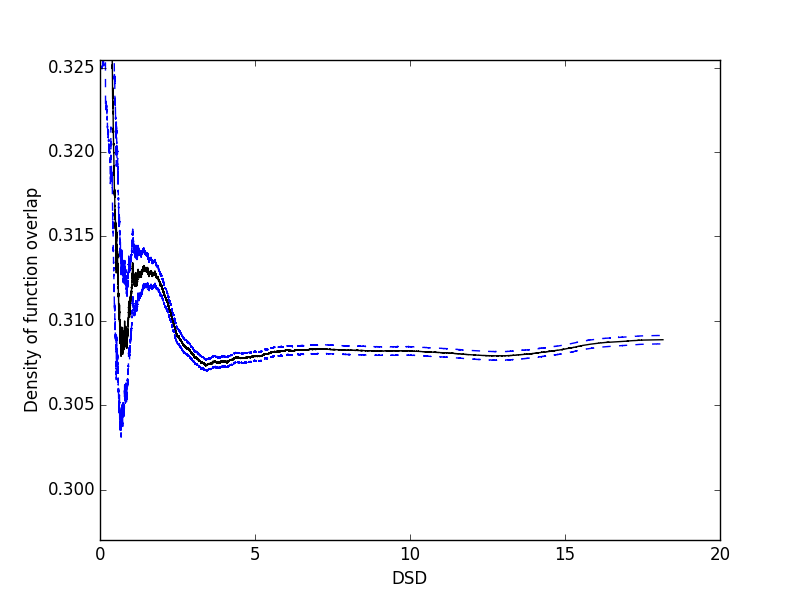
\includegraphics[width=0.333333333333\textwidth]{plots/mouse_dsd_density_randomized.png}
}
\subfloat[DSD vs Overlap, Pairs]{
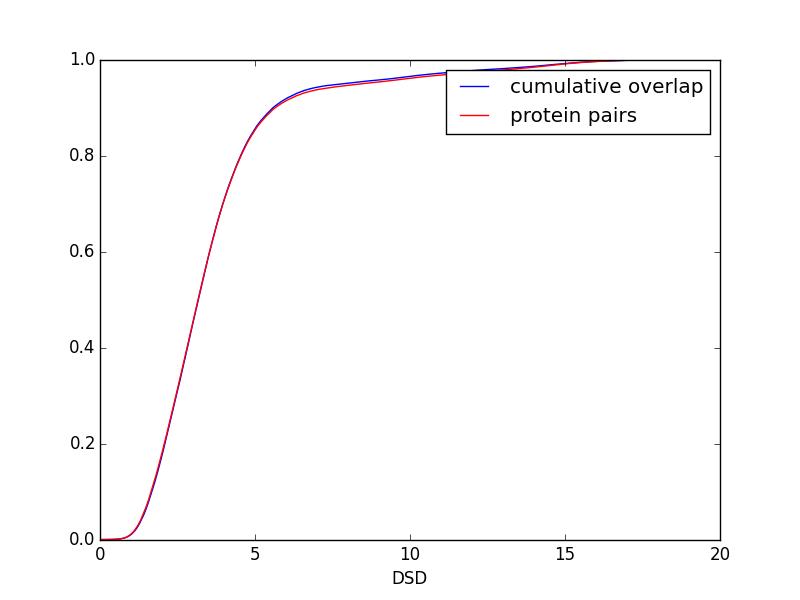
\includegraphics[width=0.333333333333\textwidth]{plots/mouse_dsd_overlap_pairs_randomized.png}
}
\subfloat[Pairs vs Cumulative Overlap]{
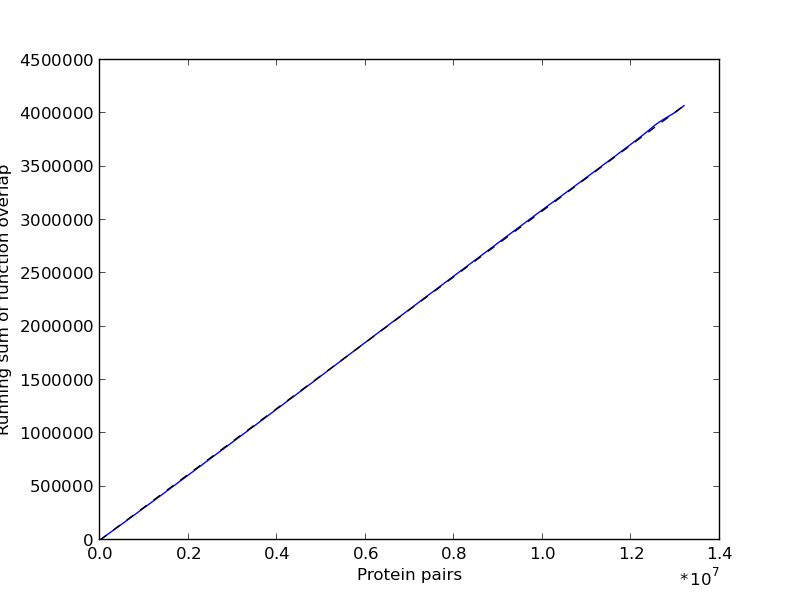
\includegraphics[width=0.333333333333\textwidth]{plots/mouse_pairs_overlap_randomized.png}
}
}
\end{figure}

\end{document}
